\lstinputlisting[language=bash,basicstyle=\small]{python_codes/fieldstone_28/keywords.ascii}

{\sl This fieldstone was developed in collaboration with Rens Elbertsen}. 
\index{contributors}{Rens Elbertsen}

The viscosity field $\eta$ is calculated as the harmonic average between a linear part $\eta_{lin}$ 
that depends on temperature only or on temperature and depth $d$ , and a non-linear,
plastic part $\eta_{plast}$ dependent on the strain rate:

\begin{equation}
\eta(T,z,\dot{\boldsymbol{\epsilon}}) = 
2 \left(\frac{1}{\eta_\text{lin}(T,z)} + \frac{1}{\eta_\text{plast}(\dot{\boldsymbol{\epsilon}})} \right)^{-1}. 
\label{eq:eta}
\end{equation}

The linear part is given by the linearized Arrhenius law (the so-called Frank-Kamenetskii approximation \cite{fran69}):

\begin{equation}
\eta_\text{lin} (T,z) = \exp(-\gamma_T T + \gamma_{z} z), \label{eq:eta_Ty}
\end{equation}

where $\gamma_T = \ln ( \Delta\eta_T)$ and $\gamma_{z}=\ln(\Delta\eta_{z})$ are parameters controlling the total viscosity 
contrast due to temperature ($\Delta\eta_T$) and pressure ($\Delta\eta_{z}$). The non-linear part is given by \cite{trha98,trha98b}: 

\begin{equation}
\eta_\text{plast} (\dot{\boldsymbol{\epsilon}}) 
= \eta^{*} + \frac{\sigma_Y}{\sqrt{\dot{\boldsymbol{\epsilon}}:\dot{\boldsymbol{\epsilon}}}}, \label{eq:eta_sigma}
\end{equation}
where $\eta^*$ is a constant representing the effective viscosity at high stresses \cite{stlh14} and $\sigma_Y$ is the yield stress, also assumed to be constant. In 2-D, the denominator in the second term of equation (\ref{eq:eta_sigma}) is given explicitly by

\begin{equation}
\sqrt{\dot{\boldsymbol{\epsilon}}:\dot{\boldsymbol{\epsilon}}} 
= \sqrt{\dot{\epsilon}_{ij} \dot{\epsilon}_{ij} } 
= \sqrt{\left( \frac{\partial u_x}{\partial x} \right)^2 + \frac{1}{2} \left( \frac{\partial u_x}{\partial y} 
+ \frac{\partial u_y}{\partial x} \right)^2 + \left( \frac{\partial u_y}{\partial y} \right)^2  }.
\end{equation}

The viscoplastic flow law (equation \ref{eq:eta}) leads to linear viscous deformation at low stresses (equation (\ref{eq:eta_Ty})) 
and to plastic deformation for stresses that exceed $\sigma_Y$ (equation (\ref{eq:eta_sigma})), with the decrease in viscosity limited by the choice of $\eta^{*}$ \cite{stlh14}.

In all cases that we present, the domain is a two-dimensional square box. The mechanical boundary conditions are for all boundaries free-slip 
with no flux across, i.e. $\tau_{xy}=\tau_{yx}=0$ and $\boldsymbol{u}\cdot \boldsymbol{n}=0$, where $\boldsymbol{n}$ denotes the outward normal to 
the boundary. Concerning the energy equation, the bottom and top boundaries are isothermal, with the temperature $T$ set to 1 and 0, respectively, 
while side-walls are assumed to be insulating, i.e. $\partial T/\partial x = 0$. The initial distribution of the temperature field is prescribed as follows:

\begin{equation}
T(x,y) = (1-y) + A \cos(\pi x)\sin(\pi y), \label{eq:initemp}
\end{equation}
where $A=0.01$ is the amplitude of the initial perturbation.


In the following Table, we list the benchmark cases according to the parameters used. 
\begin{center}
\begin{tabular}{c c c c c c c} 
\hline
Case & $Ra$ & $\Delta\eta_T$ & $\Delta\eta_y$ & $\eta^*$ & $\sigma_Y$ & Convective regime \\
\hline
1   & $10^2$ & $10^5$    & 1  & -- & --             & Stagnant lid    \\
2   & $10^2$ & $10^5$    & 1  & $10^{-3}$ & 1       & Mobile lid \\
3   & $10^2$ & $10^5$    & 10 & --  & --            & Stagnant lid \\
4   & $10^2$ & $10^5$    & 10 & $10^{-3}$ & 1       & Mobile lid  \\
5a  & $10^2$ & $10^5$    & 10 & $10^{-3}$ & 4       & Periodic  \\
5b  & $10^2$ & $10^5$    & 10 & $10^{-3}$ & 3 -- 5  & Mobile lid -- Periodic -- Stagnant lid \\
\hline
\end{tabular}\\
{\small Benchmark cases and corresponding parameters.} 
\end{center}

In Cases 1 and 3 the viscosity is directly calculated from equation (\ref{eq:eta_Ty}), while for Cases 2, 4, 5a, and 5b, we used equation (\ref{eq:eta}). For a given mesh resolution, Case 5b requires running simulations with yield stress varying between 3 and 5


In all tests, the reference Rayleigh number is set at the surface ($y=1$) to $10^2$, and the viscosity contrast due to temperature $\Delta\eta_T$ is $10^5$, implying therefore a maximum effective Rayleigh number of $10^7$ for $T=1$. Cases 3, 4, 5a, and 5b employ in addition a depth-dependent rheology with viscosity contrast  $\Delta\eta_z=10$. Cases 1 and 3 assume a linear viscous rheology that leads to a stagnant lid regime. Cases 2 and 4 assume a viscoplastic rheology that leads instead to a mobile lid regime. Case 5a also assumes a viscoplastic rheology but a higher yield stress, which ultimately causes the emergence of a strictly periodic regime. The setup of Case 5b is identical to that of Case 5a but the test consists in running several simulations using different yield stresses. Specifically, we varied $\sigma_Y$ between 3 and 5 in increments of 0.1 in order to identify the values of the yield stress corresponding to the transition from mobile to periodic and from periodic to stagnant lid regime. 

NOTE: no crank-nicolson scheme for temperature !!

%---------------------------------------------------------------------------------
\subsubsection*{Case 0: Newtonian case, a la Blankenbach et al., 1989}

\includegraphics[width=5cm]{python_codes/fieldstone_28/results_case0/vrms.pdf}
\includegraphics[width=5cm]{python_codes/fieldstone_28/results_case0/Nu.pdf}
\includegraphics[width=5cm]{python_codes/fieldstone_28/results_case0/vrms_Nu.pdf}

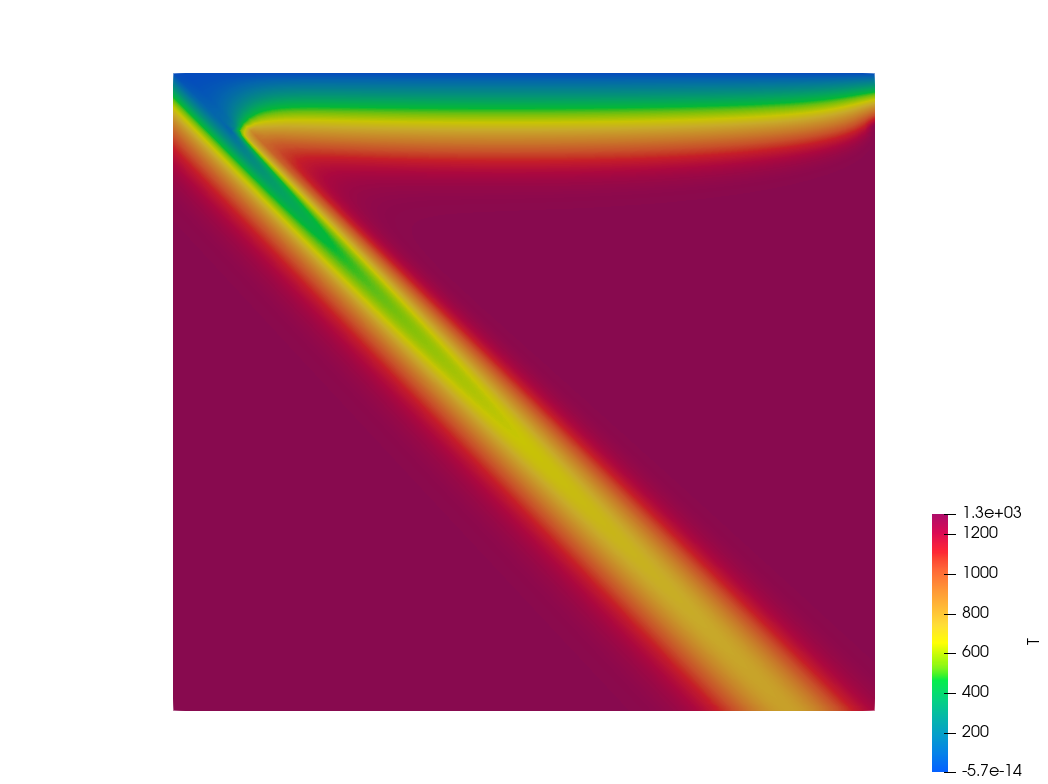
\includegraphics[width=5cm]{python_codes/fieldstone_28/results_case0/temp}
\includegraphics[width=5cm]{python_codes/fieldstone_28/results_case0/vel}



\newpage %-------------------------------------------------------
\subsubsection*{Case 1}

In this case $\eta^\star=0$ and $\sigma_Y=0$ so that $\eta_{plast}$ can be discarded.
The CFL number is set to 0.5 and the viscosity is given by 
$\eta(T,z,\dot{\boldsymbol{\epsilon}}) =   \eta_\text{lin}(T,z) $.
And since $\Delta \eta_z=1$ then $\gamma_z=0$ so that
$\eta_\text{lin} (T,z) = \exp(-\gamma_T T )$

\begin{center}
\includegraphics[width=16cm]{python_codes/fieldstone_28/results_case1/tosn15b}
\end{center}

\begin{center}
\includegraphics[width=7.8cm]{python_codes/fieldstone_28/results_case1/vrms.pdf}
\includegraphics[width=7.8cm]{python_codes/fieldstone_28/results_case1/Nu.pdf}\\
\includegraphics[width=7.8cm]{python_codes/fieldstone_28/results_case1/vrms_Nu.pdf}
\includegraphics[width=7.8cm]{python_codes/fieldstone_28/results_case1/Tavrg.pdf}
\end{center}

\begin{center}
\includegraphics[width=5cm]{python_codes/fieldstone_28/results_case1/T_profile.pdf}
\includegraphics[width=5cm]{python_codes/fieldstone_28/results_case1/eta_profile.pdf}
\includegraphics[width=5cm]{python_codes/fieldstone_28/results_case1/V_profile.pdf}
\end{center}
\newpage
\begin{center}
\includegraphics[width=7.cm]{python_codes/fieldstone_28/results_case1/u}
\includegraphics[width=7.cm]{python_codes/fieldstone_28/results_case1/v}\\
\includegraphics[width=7.cm]{python_codes/fieldstone_28/results_case1/vel}
\includegraphics[width=7.cm]{python_codes/fieldstone_28/results_case1/T}\\
\includegraphics[width=7.cm]{python_codes/fieldstone_28/results_case1/rho}
\includegraphics[width=7.cm]{python_codes/fieldstone_28/results_case1/mueff}
\end{center}









\newpage %-------------------------------------------------------
\subsubsection*{Case 2}

\includegraphics[width=16cm]{python_codes/fieldstone_28/results_case4/tosn15}

\begin{center}
\includegraphics[width=7.8cm]{python_codes/fieldstone_28/results_case2/vrms.pdf}
\includegraphics[width=7.8cm]{python_codes/fieldstone_28/results_case2/Nu.pdf}\\
\includegraphics[width=7.8cm]{python_codes/fieldstone_28/results_case2/vrms_Nu.pdf}
\includegraphics[width=7.8cm]{python_codes/fieldstone_28/results_case2/Tavrg.pdf}
\end{center}

\begin{center}
\includegraphics[width=5cm]{python_codes/fieldstone_28/results_case2/T_profile.pdf}
\includegraphics[width=5cm]{python_codes/fieldstone_28/results_case2/eta_profile.pdf}
\includegraphics[width=5cm]{python_codes/fieldstone_28/results_case2/V_profile.pdf}
\end{center}

\newpage
\begin{center}
\includegraphics[width=7.cm]{python_codes/fieldstone_28/results_case2/u}
\includegraphics[width=7.cm]{python_codes/fieldstone_28/results_case2/v}\\
\includegraphics[width=7.cm]{python_codes/fieldstone_28/results_case2/vel}
\includegraphics[width=7.cm]{python_codes/fieldstone_28/results_case2/T}\\
\includegraphics[width=7.cm]{python_codes/fieldstone_28/results_case2/rho}
\includegraphics[width=7.cm]{python_codes/fieldstone_28/results_case2/mueff}
\end{center}




\newpage %-------------------------------------------------------
\subsubsection*{Case 3}

\includegraphics[width=16cm]{python_codes/fieldstone_28/results_case3/tosn15}

\begin{center}
\includegraphics[width=7.8cm]{python_codes/fieldstone_28/results_case3/vrms.pdf}
\includegraphics[width=7.8cm]{python_codes/fieldstone_28/results_case3/Nu.pdf}\\
\includegraphics[width=7.8cm]{python_codes/fieldstone_28/results_case3/vrms_Nu.pdf}
\includegraphics[width=7.8cm]{python_codes/fieldstone_28/results_case3/Tavrg.pdf}
\end{center}

\begin{center}
\includegraphics[width=5cm]{python_codes/fieldstone_28/results_case3/T_profile.pdf}
\includegraphics[width=5cm]{python_codes/fieldstone_28/results_case3/eta_profile.pdf}
\includegraphics[width=5cm]{python_codes/fieldstone_28/results_case3/V_profile.pdf}
\end{center}

\newpage
\begin{center}
\includegraphics[width=7.cm]{python_codes/fieldstone_28/results_case3/u}
\includegraphics[width=7.cm]{python_codes/fieldstone_28/results_case3/v}\\
\includegraphics[width=7.cm]{python_codes/fieldstone_28/results_case3/vel}
\includegraphics[width=7.cm]{python_codes/fieldstone_28/results_case3/T}\\
\includegraphics[width=7.cm]{python_codes/fieldstone_28/results_case3/rho}
\includegraphics[width=7.cm]{python_codes/fieldstone_28/results_case3/mueff}
\end{center}




\newpage %-------------------------------------------------------
\subsubsection*{Case 4}

\includegraphics[width=16cm]{python_codes/fieldstone_28/results_case4/tosn15}

\begin{center}
\includegraphics[width=7.8cm]{python_codes/fieldstone_28/results_case4/vrms.pdf}
\includegraphics[width=7.8cm]{python_codes/fieldstone_28/results_case4/Nu.pdf}\\
\includegraphics[width=7.8cm]{python_codes/fieldstone_28/results_case4/vrms_Nu.pdf}
\includegraphics[width=7.8cm]{python_codes/fieldstone_28/results_case4/Tavrg.pdf}
\end{center}

\begin{center}
\includegraphics[width=5cm]{python_codes/fieldstone_28/results_case4/T_profile.pdf}
\includegraphics[width=5cm]{python_codes/fieldstone_28/results_case4/eta_profile.pdf}
\includegraphics[width=5cm]{python_codes/fieldstone_28/results_case4/V_profile.pdf}
\end{center}

\newpage
\begin{center}
\includegraphics[width=7.cm]{python_codes/fieldstone_28/results_case4/u}
\includegraphics[width=7.cm]{python_codes/fieldstone_28/results_case4/v}\\
\includegraphics[width=7.cm]{python_codes/fieldstone_28/results_case4/vel}
\includegraphics[width=7.cm]{python_codes/fieldstone_28/results_case4/T}\\
\includegraphics[width=7.cm]{python_codes/fieldstone_28/results_case4/rho}
\includegraphics[width=7.cm]{python_codes/fieldstone_28/results_case4/mueff}
\end{center}

\newpage %-------------------------------------------------------
\subsubsection*{Case 5a - Periodic Solutions}

\begin{center}
\includegraphics[width=7.8cm]{python_codes/fieldstone_28/results_case5/vrms.pdf}
\includegraphics[width=7.8cm]{python_codes/fieldstone_28/results_case5/Nu.pdf}\\
\includegraphics[width=7.8cm]{python_codes/fieldstone_28/results_case5/vrms_Nu.pdf}
\includegraphics[width=7.8cm]{python_codes/fieldstone_28/results_case5/Tavrg.pdf}\\
\includegraphics[width=7.8cm]{python_codes/fieldstone_28/results_case5/u.pdf}
\includegraphics[width=7.8cm]{python_codes/fieldstone_28/results_case5/v.pdf}
\end{center}


\newpage
\noindent
\begin{center}
\includegraphics[width=3.74cm]{python_codes/fieldstone_28/results_case5/T_0000}
\includegraphics[width=3.74cm]{python_codes/fieldstone_28/results_case5/T_0010}
\includegraphics[width=3.74cm]{python_codes/fieldstone_28/results_case5/T_0020}
\includegraphics[width=3.74cm]{python_codes/fieldstone_28/results_case5/T_0030}\\
\includegraphics[width=3.74cm]{python_codes/fieldstone_28/results_case5/T_0040}
\includegraphics[width=3.74cm]{python_codes/fieldstone_28/results_case5/T_0050}
\includegraphics[width=3.74cm]{python_codes/fieldstone_28/results_case5/T_0060}
\includegraphics[width=3.74cm]{python_codes/fieldstone_28/results_case5/T_0070}\\
\includegraphics[width=3.74cm]{python_codes/fieldstone_28/results_case5/T_0080}
\includegraphics[width=3.74cm]{python_codes/fieldstone_28/results_case5/T_0090}
\includegraphics[width=3.74cm]{python_codes/fieldstone_28/results_case5/T_0100}
\includegraphics[width=3.74cm]{python_codes/fieldstone_28/results_case5/T_0110}\\
\includegraphics[width=3.74cm]{python_codes/fieldstone_28/results_case5/T_0120}
\includegraphics[width=3.74cm]{python_codes/fieldstone_28/results_case5/T_0130}
\includegraphics[width=3.74cm]{python_codes/fieldstone_28/results_case5/T_0140}
\includegraphics[width=3.74cm]{python_codes/fieldstone_28/results_case5/T_0150}\\
{\captionfont Temperature field evolution}
\end{center}

%-----------------------------------------------
\subsubsection*{Case 5b - Bifurcation Analysis}

Case 5b is an extension of Case 5a. Here we varied the yield stress from $\sigma_Y=$ 3 to 5 with the goal of identifying 
the critical values at which the system transitions from a steady, mobile lid regime (for low values of $\sigma_Y$ ),
to a periodic regime first (for intermediate values of $\sigma_Y$ ), and to a steady, stagnant lid regime afterward (for
high values of $\sigma_Y$).

\todo[inline]{Carry out all these runs and plot against paper data}

